%\subsection{Experimental Setup}
%\indent \textbf{Participants.}

\indent \textbf{Participants.} Thirty-two healthy participants (aged 21--45 years, 14 men) took part in the
experiment. All participants gave written informed consent to participation and the experimental protocol was approved by the local ethics committee (protocol: GR\_08\_20170428). Three participants were excluded from data analysis due to incomplete data or difficulties in complying with the task requirements.

%\indent \textbf{The Invisible Maze Task.} 
\indent \textbf{The Invisible Maze Task.} Participants freely explored an interactive sparse invisible maze environment by walking and probing for virtual visual wall feedback with their hand, delivered by a virtual reality (VR) headset. Four different mazes (Fig. \ref{imt_task} B) were explored in three consecutive runs. Upon collision of the hand with an invisible wall, an illuminated white disc was displayed 30cm behind the collision point parallel to the invisible wall (Fig. \ref{imt_task} C). Due to the complexity of the technical details, please consult~\cite{gehrke2018}. In summary, the task required participants to explore mazes to build a spatial representation of the maze layout.%This behavior is comparable to explorative wall touches in the dark to find your way.

\begin{figure}[h]
\centering
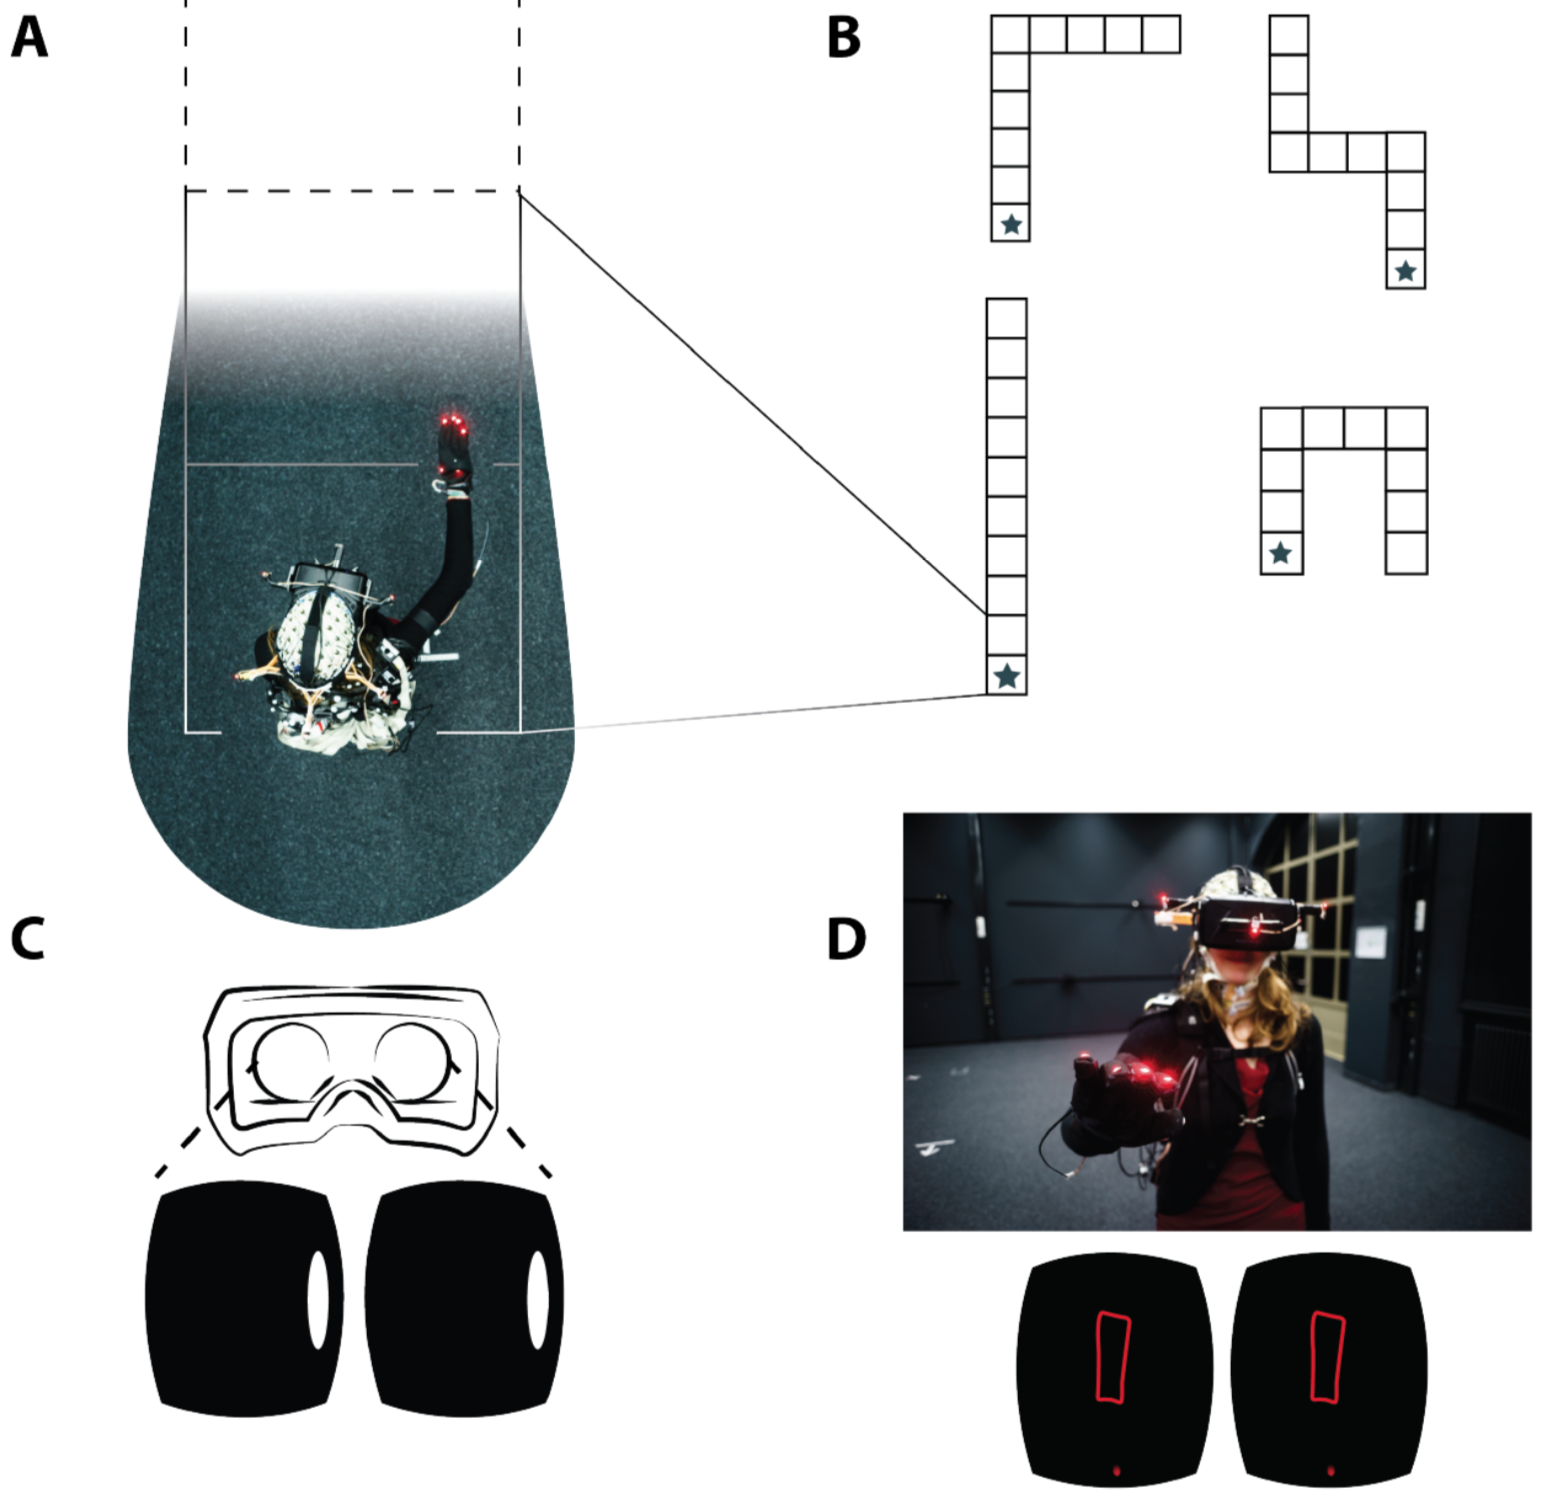
\includegraphics[width=\linewidth]{IMT_Task.png}
\vspace{0pt}
\caption{Invisible Maze Task, \textbf{A} Participant from a bird’s eye view. \textbf{B} Participants are instructed to explore four different mazes and return to the start. \textbf{C} First-person view in binocular ""VR optics"" of a wall touch. \textbf{D} Top: Participants draw a top-down view of the explored maze. Participant is equipped with 160 channels wireless EEG, head-mounted virtual reality goggles and LEDs for motion capture. Bottom: drawn sketch map. Find a detailed description in~\cite{gehrke2018}.}
\label{imt_task}
\end{figure}

<<<<<<< Updated upstream
\subsection{Statistical Analyses}
We computed an ordinary logistic regression entering each participants IPQ general presence score as the ordinary scaled dependent variable. For the predictors, we first computed the participant average and then entered, Duration, Number of Touches, Sketchmap,  \todo{add all predictors used} into the regression model. For an explanation of each variable, pleas consult~\cite{gehrke2018}. To assess the predictive accuracy of the model, we ran leave-one-out-cross-validation (LOOCV) \todo{add LOOCV citation}. All statistical analyses were conducted using R, \todo{add version and packages citations}. The code and data are available online \todo{add link to data repository and analyses code}.
=======
\indent \textbf{Assessing experienced presence.} In the current work, we were interested in the subjectively reported experience of presence. Therefore we analyzed the first item on Igroup's presence questionnaire, i.e. 'In the computer generated world I had a sense of "being there"' rated from 'not at all' to 'very much'~\cite{ipq, slaterQ1}.

\indent \textbf{Statistical Analyses.} We computed an ordinary least squares regression entering IPQ presence score as the dependent variable using R~\cite{rver}. For the predictors, we first computed the participant average and then entered: movement velocity, time-on-task, number of wall touches, sketch map accuracy, video game experience, sex, perspective taking and orientation ability, sense of direction into the regression model. For an explanation of each predictor, pleas consult~\cite{gehrke2018}. To reduce over-fitting and increase the possible insight of our results for other researcher, a stepwise model selection procedure based on Akaike's information criterion (AIC) was computed using 'stepAIC' of package 'MASS'~\cite{aic, mass}.
Ultimately, the reduced model of three predictors was assessed in terms of the predictive accuracy of the model. Therefore, a cross-validation with 5 folds was computed to obtain a robust mean absolute error~\cite{cv, mae}. With 29 participants comprising the analyzed data, each training fold consisted of either 23 or 24 participants with either 5 or 6 participants in the evaluated test fold.

% The code and data are available online \todo{add link to data repository and analyses code}
>>>>>>> Stashed changes
